\clearpage
\appendix
\chapter{Parelles Model-Text utilitzades als experiments}
\label{sec:parelles_model_text}

En aquest apèndix es recullen les difents parelles model-text utilitzades en els experiment de la secció \ref{cha:experiments}. Els quatre primers provenen de la col·lecció ``BPMN For Research'' de Camunda \cite{camunda_models}. Els quatre següents s'han convertit manualment a bpmn a partir del conjunt de dades d'exemple de \cite{text2process_models} utilitzant el software de modelat de BPMN de Camunda, \emph{bpmn.io}. L'exemple: ``Hospital'', s'ha obtingut de l'article disponible a \cite{hospital_ref}. Pel que fa a l'última parella model-text, ``Zoo'', aquesta s'ha modelat manualment a partir de l'explicació d'un cas real de procés de negoci al Zoo de Barcelona\footnote{Les fonts de les quals s'ha obtingut la descripció del procés de negoci no són oficials. Per aquest fet, aquest procés es considerarà com un exemple acadèmic.}.

Per facilitar la lectura d'aquest imprès s'han inclòs els diagrames BPMN ampliats en fulls apaisats al final d'aquest annex.

\clearpage
\section{Credit Scoring \texttt{[CRED]} }

\subsection*{Descripció textual}

\textit{The sales clerks in a bank can use their software frontend to receive the credit-scoring for a certain customer. This starts a process in the banking system which communicates with the agency in the background. This process sends a scoring request to the agency right after the beginning. Then, the Agency does a first quick scoring (level 1). This will often lead to an immediate result which is then returned directly to the banking system within seconds. The banking process presents the result to the clerk sitting at the frontend. Sometimes the scoring cannot be determined immediately and takes longer. In this case the agency informs the banking process of the delay and then starts the level 2 scoring (which can take up to a couple of minutes). After the scoring result is determined, the information is sent back to the banking process. The banking process displays a message to the clerk when he receives information about the delay to check again later. As soon as the result arrives, it can be seen at the frontend.}

\subsection*{Model BPMN}

\begin{figure}[!h]
    \centering
    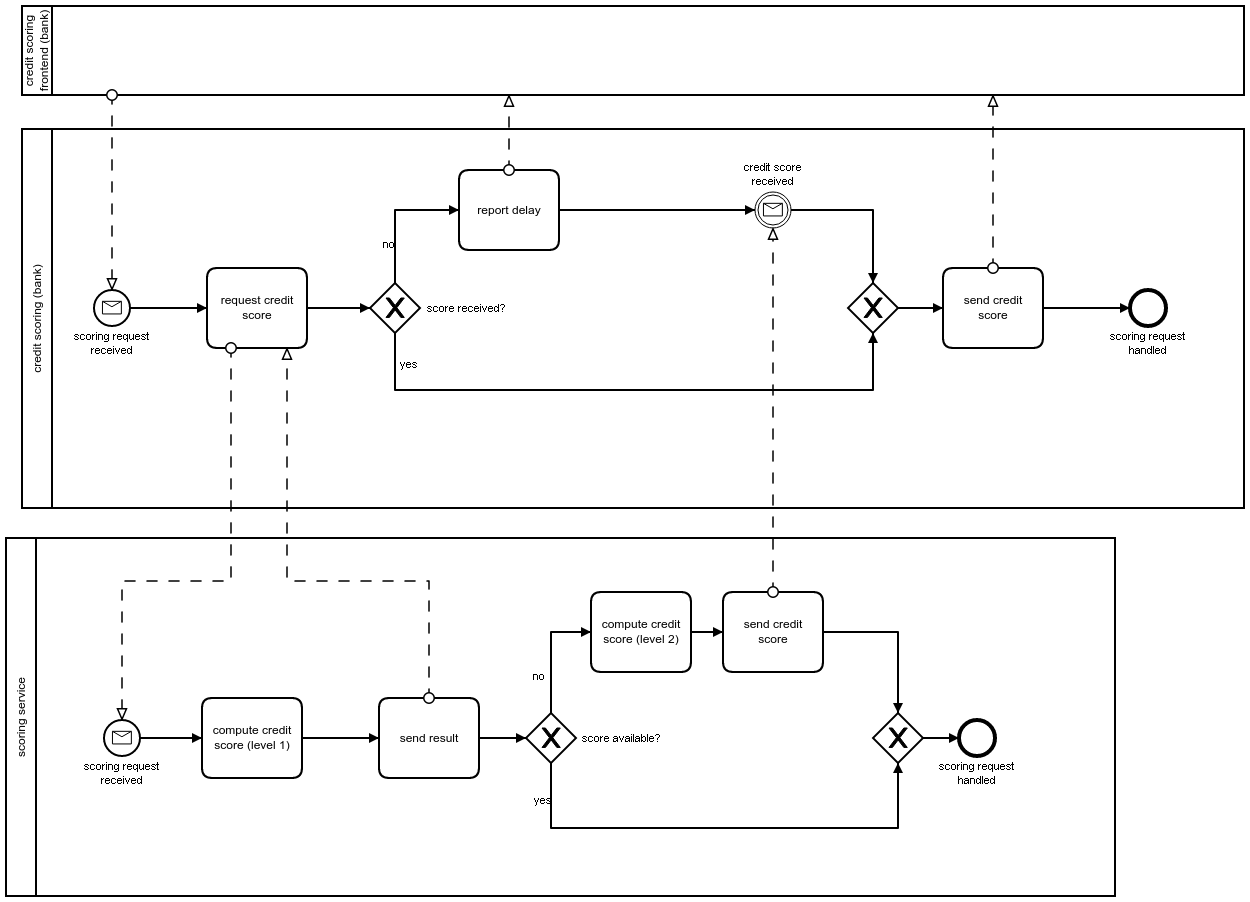
\includegraphics[width=\textwidth]{figures/benchmark/Credit-scoring.png}
\end{figure}

\clearpage
%-------------------------

\section{Self Service Restaurant \texttt{[REST]}}

\subsection*{Descripció textual}

\textit{A guest enters the restaurant when feeling hungry. He chooses a dish from the changing meal range and waits until it is his turn. Following this he places his order with the employee. The employee enters the order into the POS system and collects the money from the guest. After the payment, the employee sets up a buzzer and passes it on to the guest with the following information: "When the buzzer rings, your dinner is ready". Afterwards the employee informs the chef of the new meal order. The chef prepares the meal and places it in the service hatch. He then informs the employee that he has placed the finished meal in the service hatch. As soon as the employee is aware that the meal is ready he sets off the guest's buzzer. This is how the guest finds out that his meal is ready for collection. He can pick up his meal and eat it. As soon as the guest appears at the service hatch, the employee hands over his meal. Should a guest not react to the buzzer, the employee calls for him after 5 minutes, if necessary several times in a row.}

\subsection*{Model BPMN}

\begin{figure}[!h]
    \centering
    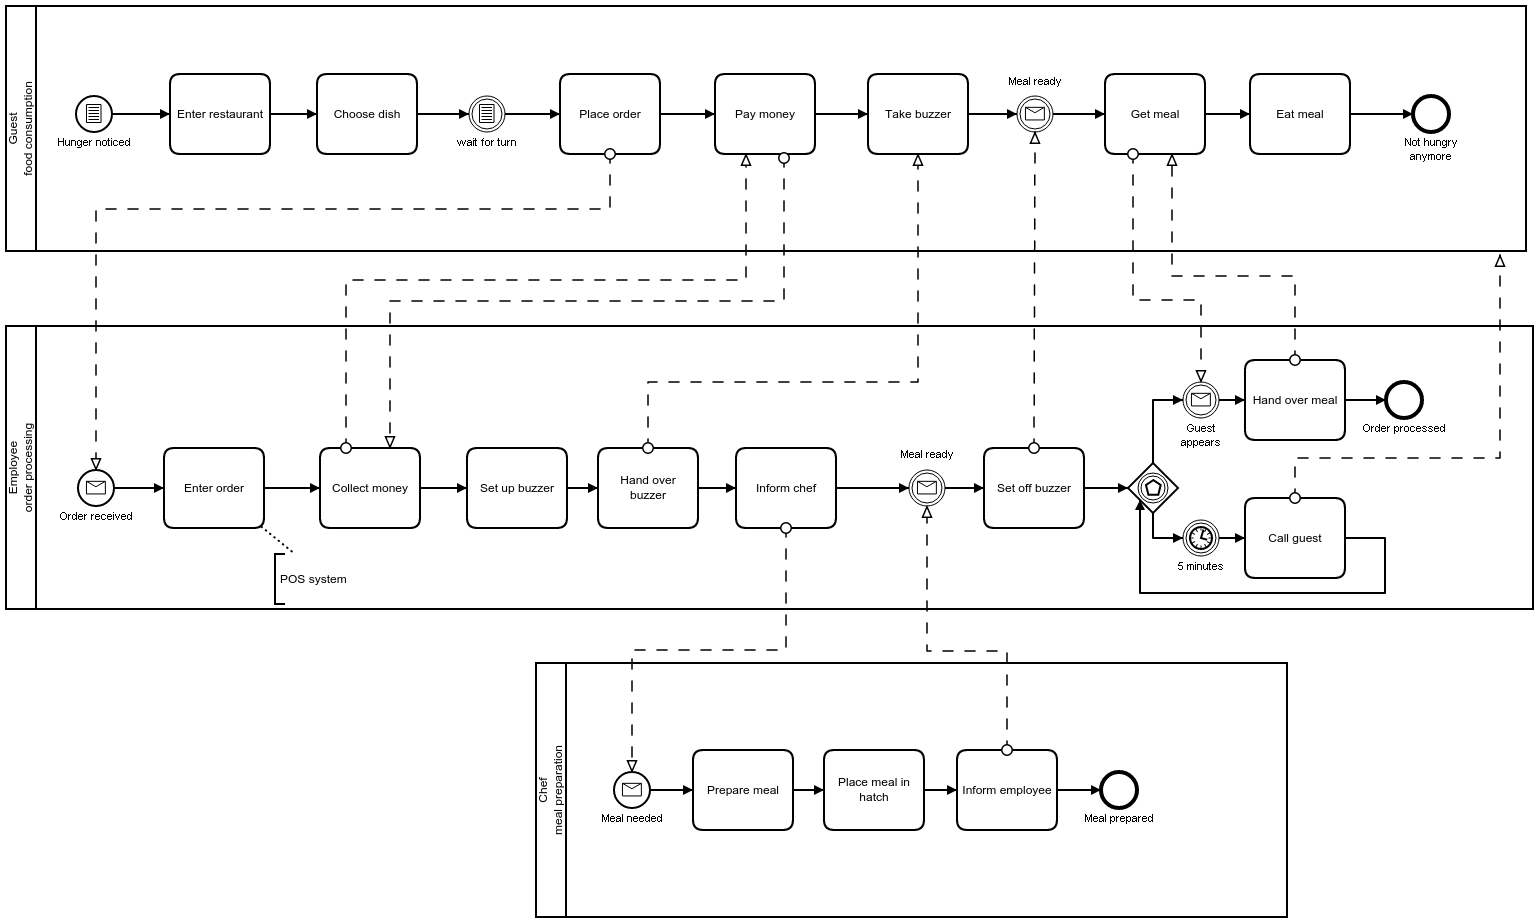
\includegraphics[width=\textwidth]{figures/benchmark/Self-service-restaurant.png}
\end{figure}

\clearpage
%-------------------------

\section{Dispatch of Goods \texttt{[DISP]}}

\subsection*{Descripció textual}

\textit{If goods shall be shipped, the secretary clarifies who will do the shipping. If you have large amounts, special shipping will be necessary. In these cases the secretary invites three logistic companies to make offers and she selects one of them. In case of small amounts, normal post shipment is used. Therefore a package label is written by the secretary and a parcel insurance taken by the logistics department head if necessary. In the meantime the goods can be already packaged by the warehousemen. If everything is ready, the packaged goods are prepared for being picked up by the logistic company.}


\subsection*{Model BPMN}

\begin{figure}[!h]
    \centering
    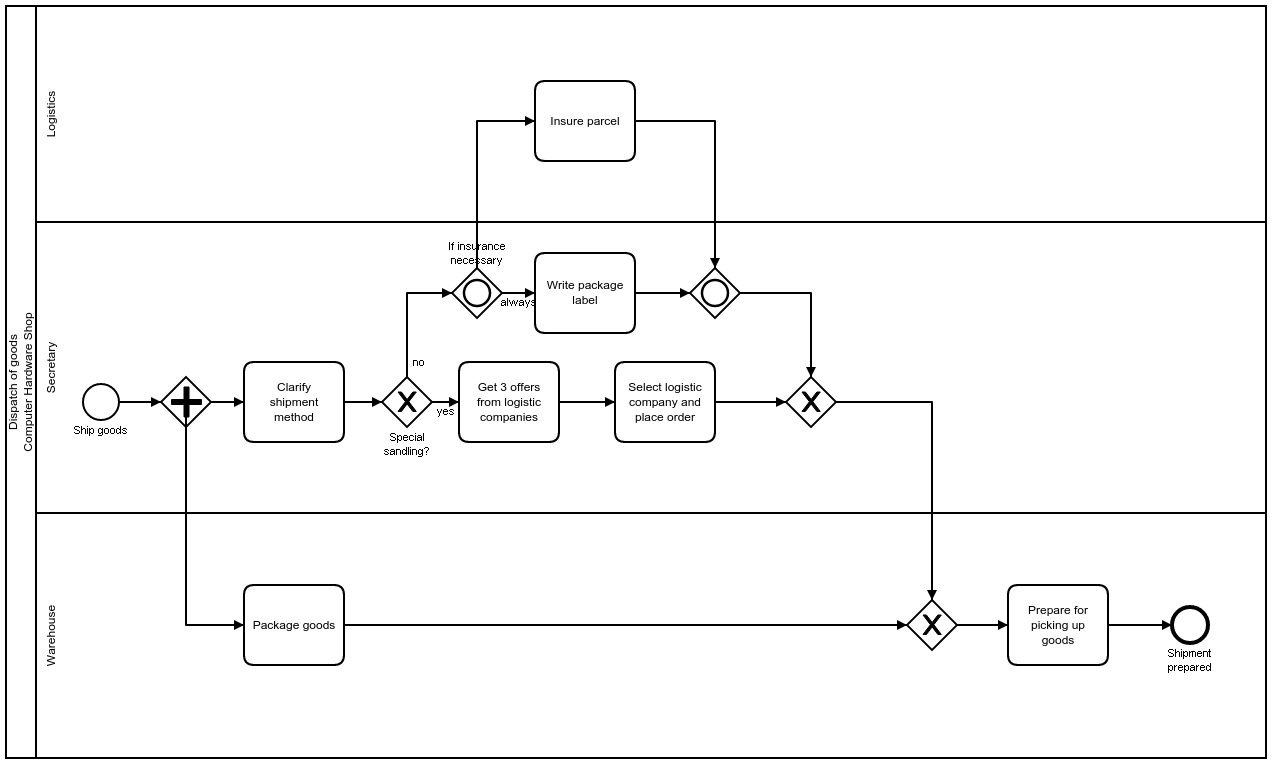
\includegraphics[width=\textwidth]{figures/benchmark/Dispatch-of-goods.png}
\end{figure}

\clearpage
%-------------------------

\section{Recourse \texttt{[RECO]}}

\subsection*{Descripció textual}

\textit{If an insurant could be possibly subrogated against, I get information about that. I check that case and if the possibility is really there, I send a request for payment to the insurant and make me a reminder. If recourse is not possible, I close the case. When we receive the money, I make a booking and close the case. If the insurant disagrees with the recourse, I’ll have to check the reasoning of that. If he is right, I simply close the case. If he is wrong, I forward the case to a collection agency. It the deadline for disagreement is reached and we haven’t received any money, I forward the case to the collection agency as well.}

\subsection*{Model BPMN}

\begin{figure}[!h]
    \centering
    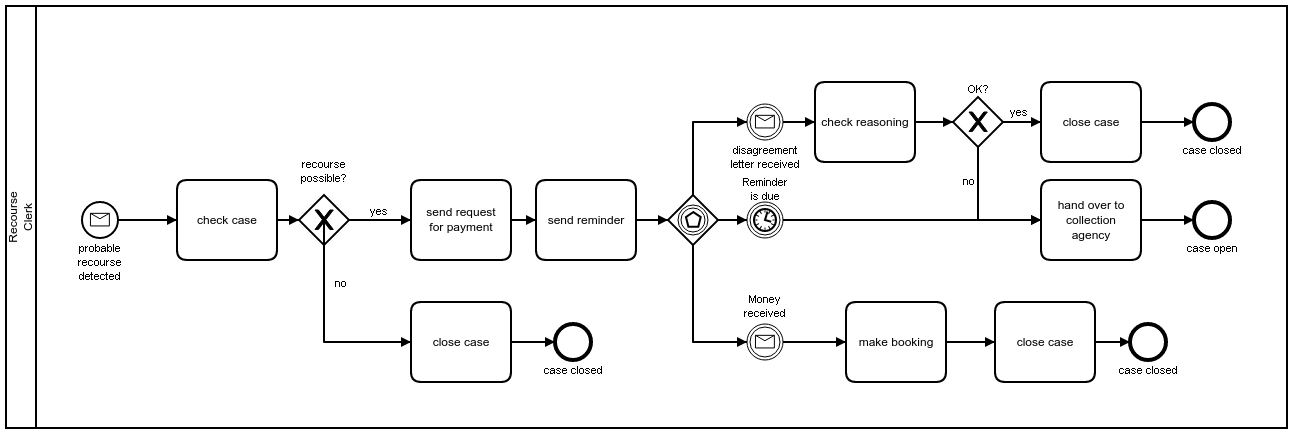
\includegraphics[width=\textwidth]{figures/benchmark/Recourse.png}
\end{figure}

\clearpage
%-------------------------

\section{Bicycle Manufacturer \texttt{[BICL]}}

\subsection*{Descripció textual}

\textit{A small company manufactures customized bicycles. Whenever the sales department receives an order, a new process instance is created. A member of the sales department can then reject or accept the order for a customized bike. In the former case, the process instance is finished. In the latter case, the storehouse and the engineering department are informed. The storehouse immediately processes the part list of the order and checks the required quantity of each part. If the part is available in-house, it is reserved. If it is not available, it is back-ordered. This procedure is repeated for each item on the part list. In the meantime, the engineering department prepares everything for the assembling of the ordered bicycle. If the storehouse has successfully reserved or back-ordered every item of the part list and the preparation activity has finished, the engineering department assembles the bicycle. Afterwards, the sales department ships the bicycle to the customer and finishes the process instance.}

\subsection*{Model BPMN}

\begin{figure}[!h]
    \centering
    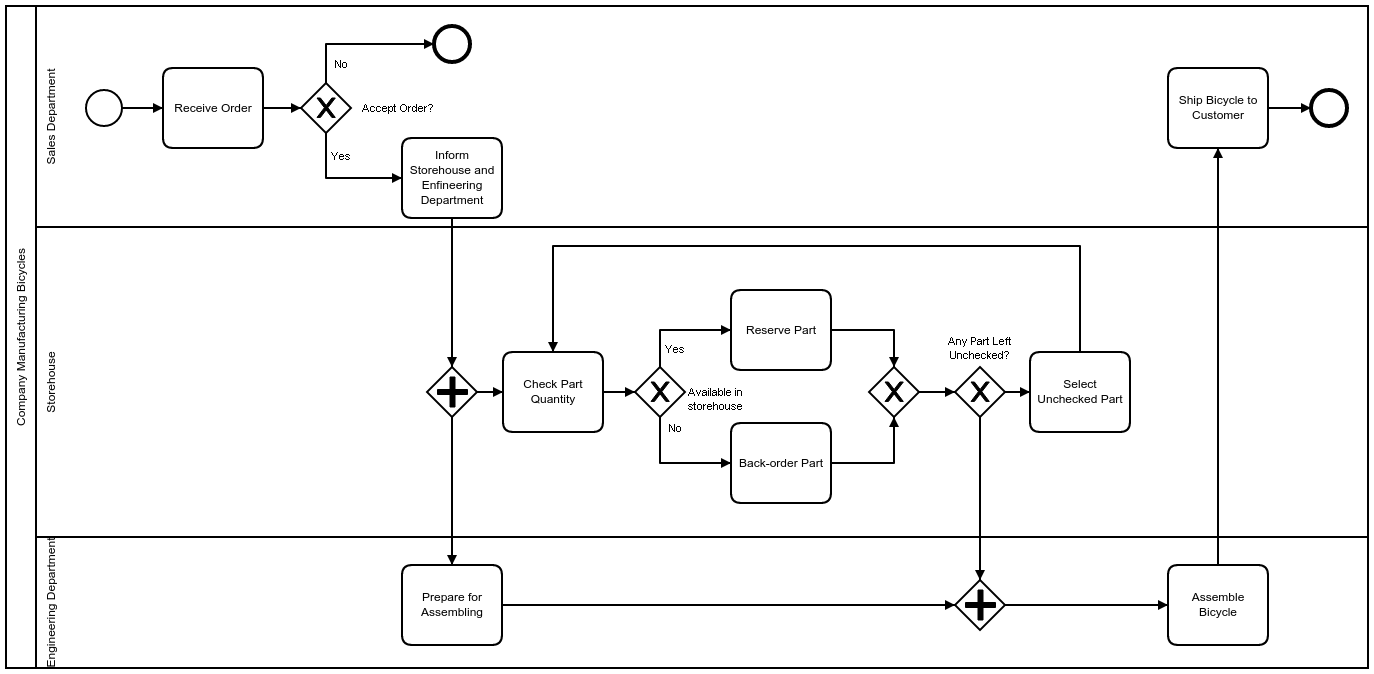
\includegraphics[width=\textwidth]{figures/benchmark/Bicycle_Manufacturer.png}
\end{figure}

\clearpage
%-------------------------


\section{Computer Repair Shop \texttt{[COMP]}}

\subsection*{Descripció textual}

\textit{The workflow of a computer repair service (CRS) can be described as follows. A customer brings in a defective computer and the CRS checks the defect and hands out a repair cost calculation back. If the customer decides that the costs are acceptable, the process continues, otherwise she takes her computer home unrepaired. The ongoing repair consists of two activities, which are executed, in an arbitrary order. The first activity is to check and repair the hardware, whereas the second activity checks and configures the software. After each of these activities, the proper system functionality is tested. If an error is detected another arbitrary repair activity is executed, otherwise the repair is finished.}

\subsection*{Model BPMN}

\begin{figure}[!h]
    \centering
    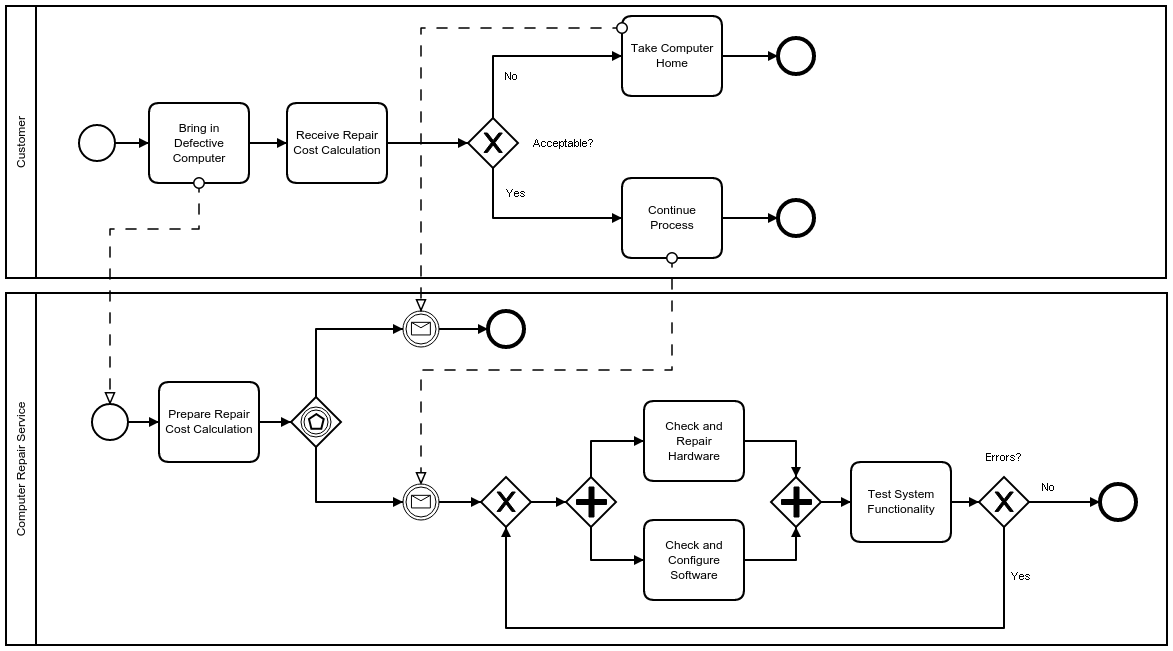
\includegraphics[width=\textwidth]{figures/benchmark/Computer_Repair.png}
\end{figure}

\clearpage
%-------------------------

\section{Hotel \texttt{[HOTL]}}

\subsection*{Descripció textual}

\textit{The Evanstonian is an upscale independent hotel. When a guest calls room service at The Evanstonian, the room-service manager takes down the order. She then submits an order ticket to the kitchen to begin preparing the food. She also gives an order to the sommelier (i.e., the wine waiter) to fetch wine from the cellar and to prepare any other alcoholic beverages. Eighty percent of room-service orders include wine or some other alcoholic beverage. Finally, she assigns the order to the waiter. While the kitchen and the sommelier are doing their tasks, the waiter readies a cart (i.e., puts a tablecloth on the cart and gathers silverware). The waiter is also responsible for nonalcoholic drinks. Once the food, wine, and cart are ready, the waiter delivers it to the guest's room. After returning to the room-service station, the waiter debits the guest's account. The waiter may wait to do the billing if he has another order to prepare or deliver.}

\subsection*{Model BPMN}

\begin{figure}[!h]
    \centering
    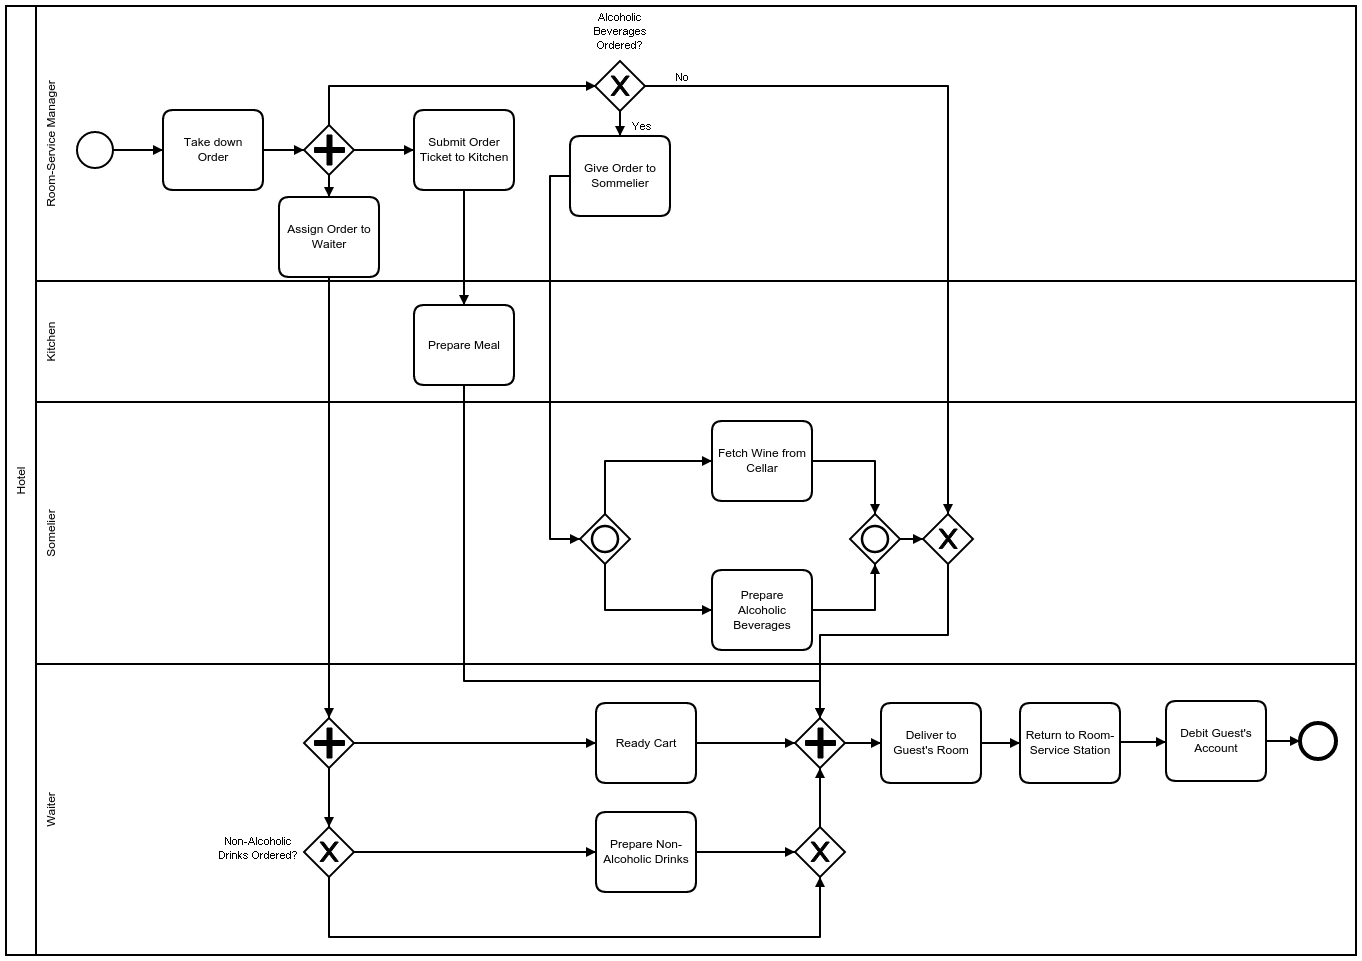
\includegraphics[width=\textwidth]{figures/benchmark/Hotel.png}
\end{figure}

\clearpage
%-------------------------

\section{Underwriter \texttt{[UNWR]}}

\subsection*{Descripció textual}

\textit{Whenever a company makes the decision to go public, its first task is to select the underwriters. Underwriters act as financial midwives to a new issue. Usually they play a triple role: First they provide the company with procedural and financial advice, then they buy the issue, and finally they resell it to the public.}

\textit{Established underwriters are careful of their reputation and will not handle a new issue unless they believe the facts have been presented fairly. Thus, in addition to handling the sale of a company's issue, the underwriters in effect give their seal of approval to it.}

\textit{They prepare a registration statement for the approval of the Securities and Exchange Commission (SEC). In addition to registering the issue with the SEC, they need to check that the issue complies with the so-called blue-sky laws of each state that regulate sales of securities within the state. While the registration statement is awaiting approval, underwriters begin to firm up the issue price. They arrange a road show to talk to potential investors. Immediately after they receive clearance from the SEC, underwriters fix the issue price. After that they enter into a firm commitment to buy the stock and then offer it to the public, when they haven't still found any reason not to do it.}

\subsection*{Model BPMN}

\begin{figure}[!h]
    \centering
    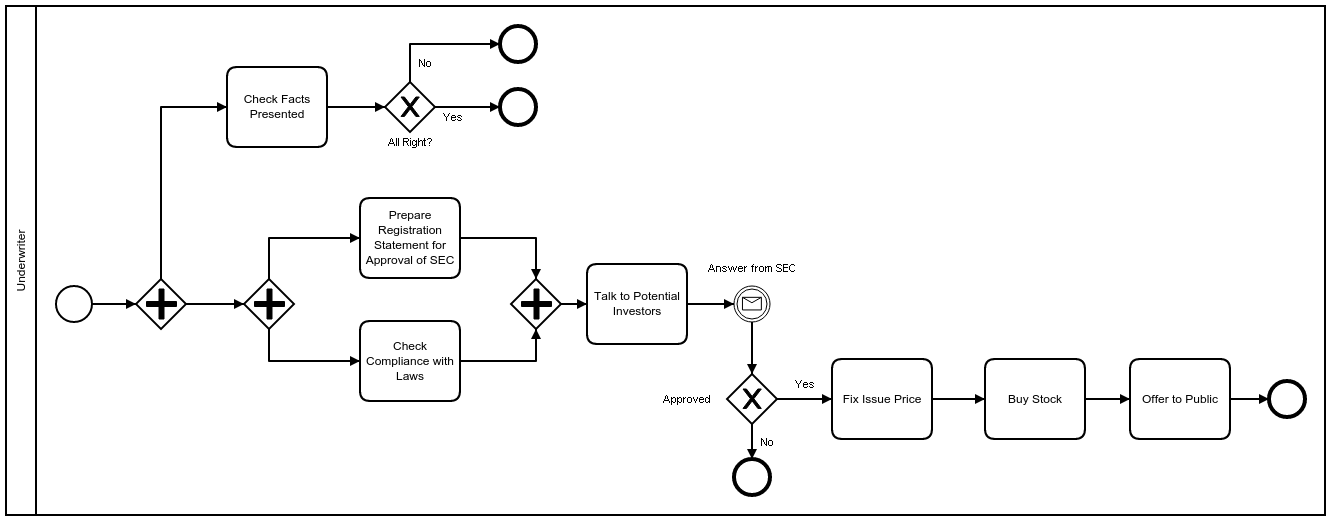
\includegraphics[width=\textwidth]{figures/benchmark/Underwriter.png}
\end{figure}

\clearpage
%-------------------------

\section{Hospital \texttt{[HOSP]}}

\subsection*{Descripció textual}

\textit{The examination process can be summarised as follows. The process starts when the female patient is examined by an outpatient physician, who decides whether she is healthy or needs to undertake an additional examination. In the former case, the physician fills out the examination form and the patient can leave. In the latter case, an examination and follow-up treatment order is placed by the physician who additionally fills out a request form. Beyond information about the patient, the request form includes details about the examination requested and refers to a suitable lab. Furthermore, the outpatient physician informs the patient about potential risks. If the patient signs an informed consent and agrees to continue with the procedure, a delegate of the physician arranges an appointment of the patient with one of the wards. The latter is then responsible for taking a sample to be analysed in the lab later. Before the appointment, the required examination and sampling is prepared by a nurse of the ward based on the information provided by the outpatient section. Then, a ward physician takes the sample requested. He further sends it to the lab indicated in the request form and conducts the follow-up treatment of the patient.  After receiving the sample, a physician of the lab validates its state and decides whether the sample can be used for analysis or whether it is contaminated and a new sample is required. After the analysis is performed by a medical technical assistant of the lab, a lab physician validates the results. Finally, a physician from the outpatient department makes the diagnosis and prescribes the therapy for the patient.}

\subsection*{Model BPMN}

\begin{figure}[!h]
    \centering
    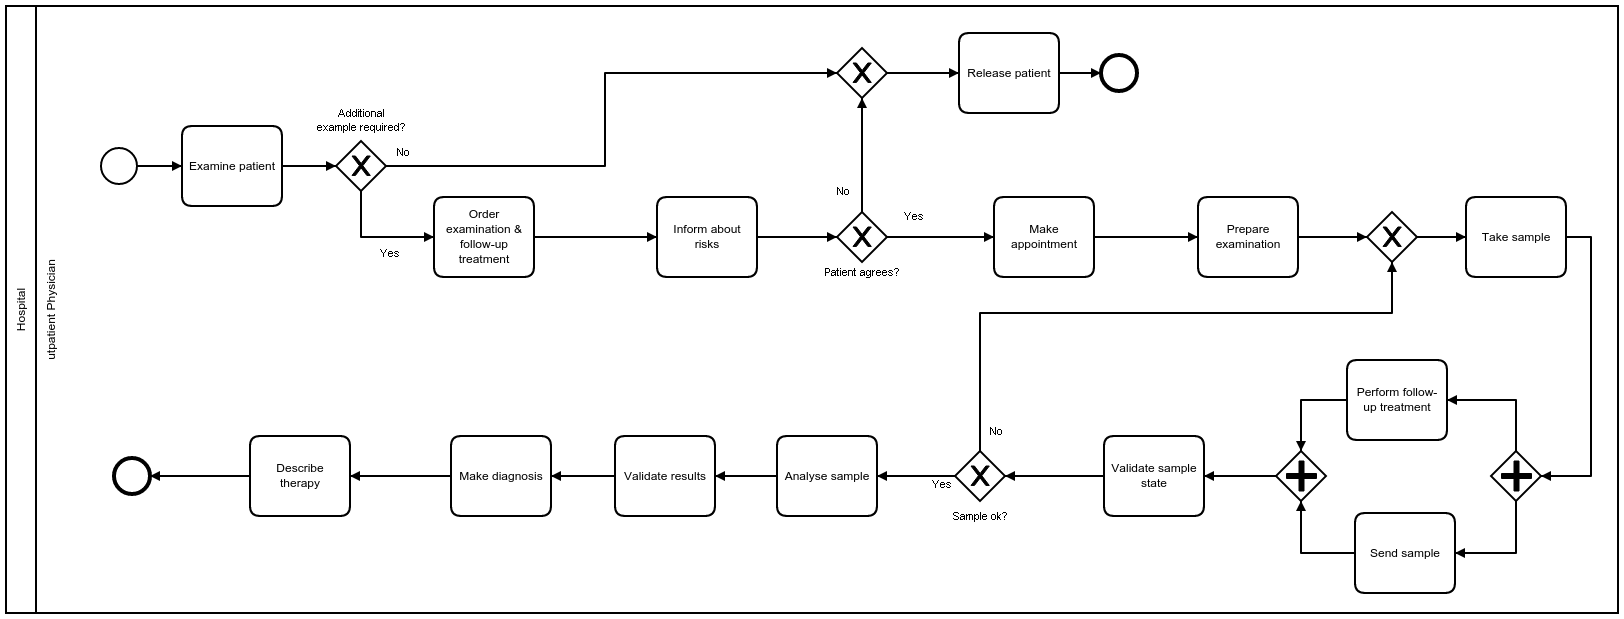
\includegraphics[width=\textwidth]{figures/benchmark/Hospital.png}
\end{figure}

\clearpage
%---------------------

\section{Zoo \texttt{[ZOO]}}
\label{sec:benchmark-zoo}

\subsection*{Descripció textual}

\textit{When a visitor wants to become a member of Barcelona's ZooClub, the following steps must be taken. First of all, the customer must decide whether he wants an individual or family membership. If he wants an individual membership, he must prepare his personal information. If he wants a family membership instead, he should prepare the information for its spouse and spawn as well. The customer must then give this information to the ZooClub department. The ZooClub department introduces the visitor's personal data into the system and takes the payment request to the Billing department. The ZooClub department also forwards the visitor's information to the marketing department. The billing department sends the payment request to the bank. The bank processes the payment information and, if everything is correct, charges the payment into user's account. Once the payment is confirmed, the ZooClub department can print the card and deliver it to the visitor. In the meantime, the Marketing department makes a request to mail the Zoo Club's magazine to the visitor's home. Once the visitor receives the card, he can go home.}

\subsection*{Model BPMN}

\begin{figure}[!h]
    \centering
    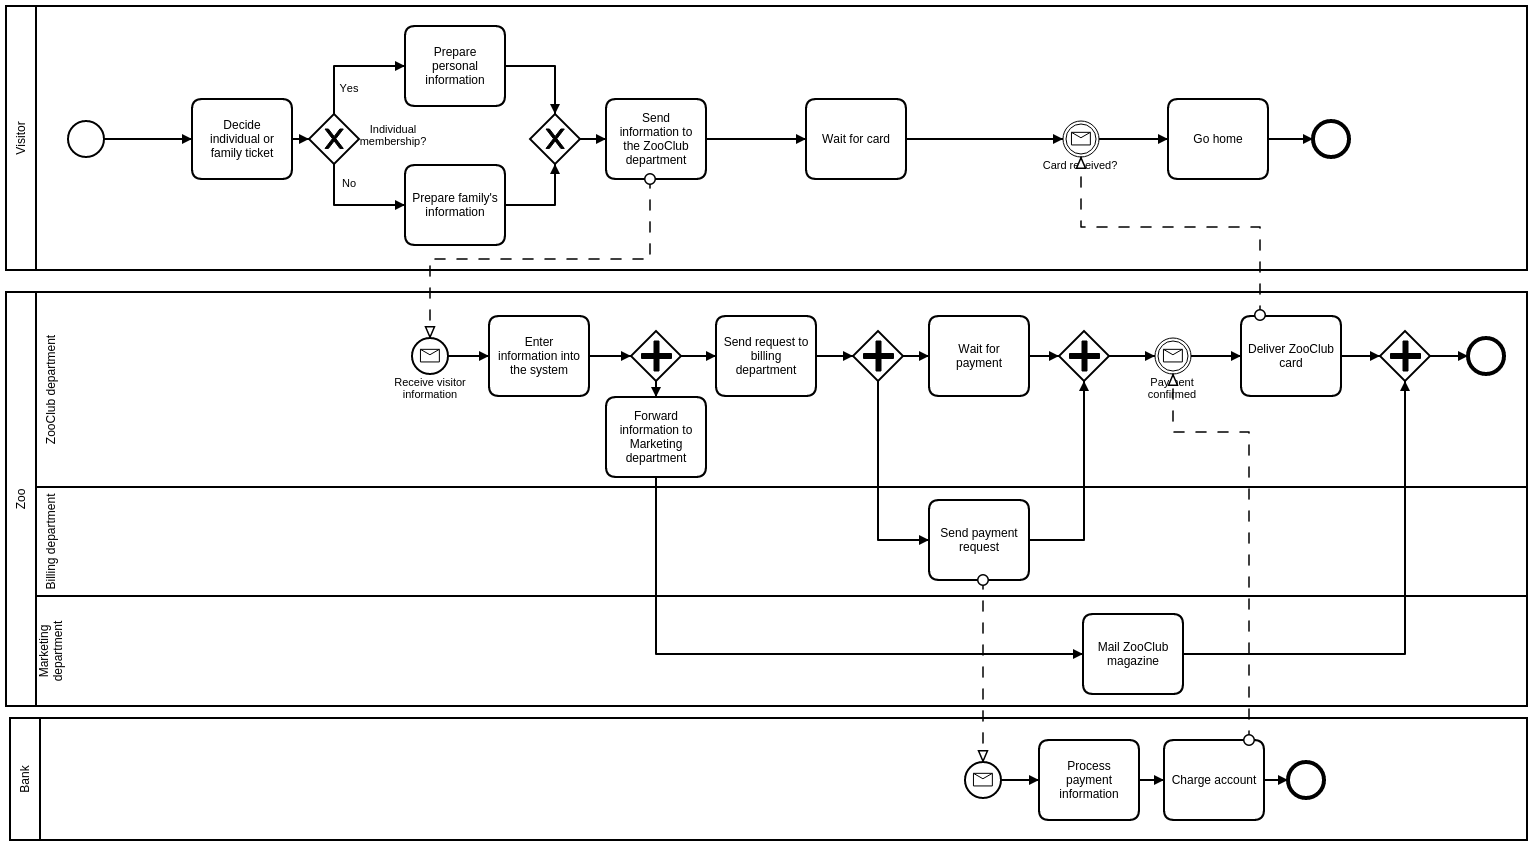
\includegraphics[width=\textwidth]{figures/benchmark/Zoo.png}
\end{figure}

\clearpage
%-------------------------

\begin{landscape}
\thispagestyle{empty}
\newgeometry{left=1cm, top=9cm}

\section*{Credit Scoring \texttt{[CRED]} }
\begin{figure}[!h]
    \centering
    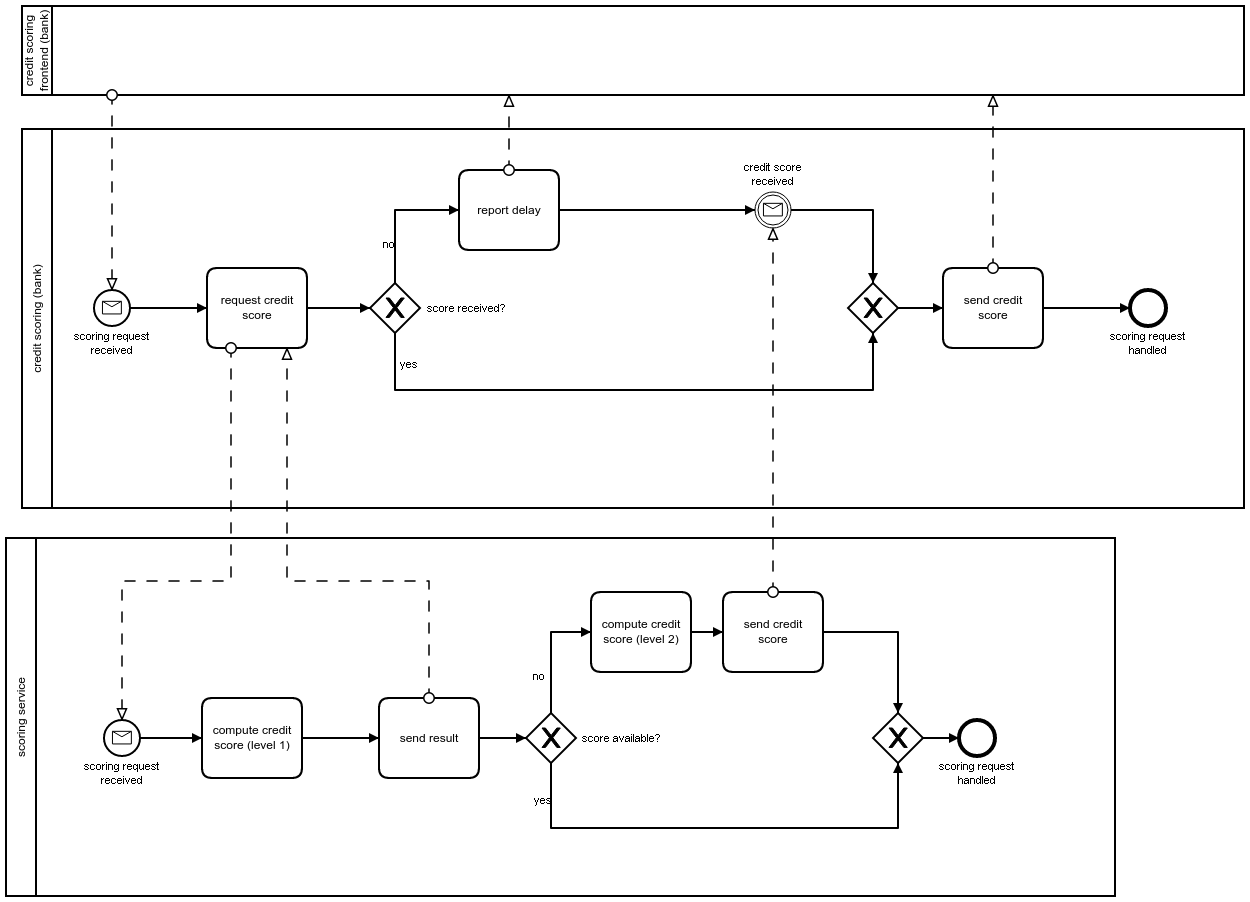
\includegraphics[width=1.3\textwidth]{figures/benchmark/Credit-scoring.png}
\end{figure}
\end{landscape}

\clearpage
%-------------------------

\begin{landscape}
\thispagestyle{empty}
\newgeometry{left=1cm, top=9cm}
\section*{Self Service Restaurant \texttt{[REST]}}

\begin{figure}[!h]
    \centering
    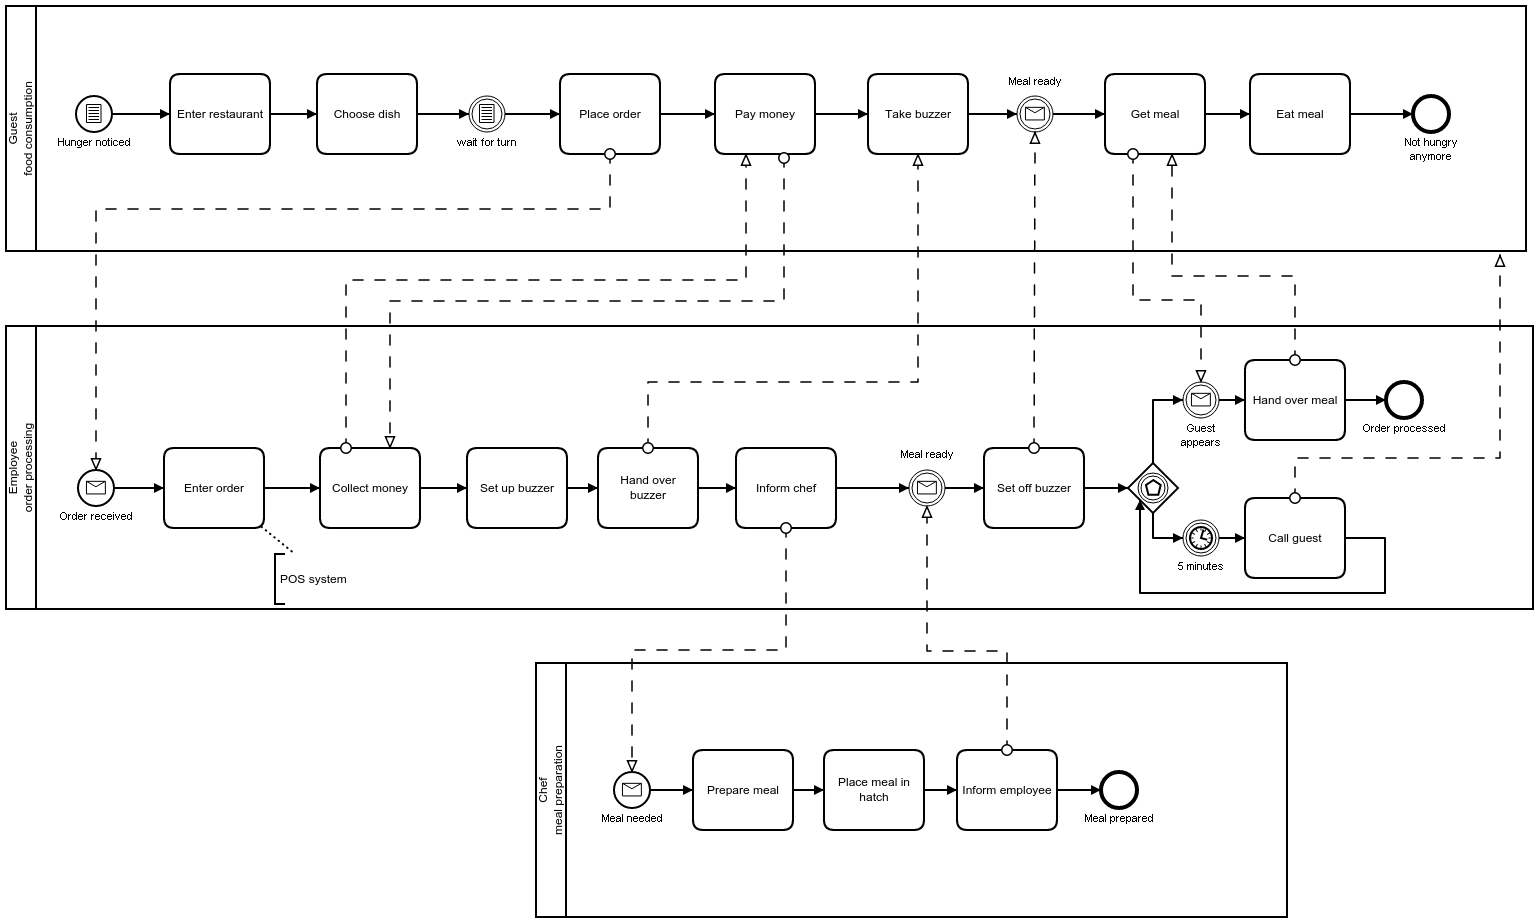
\includegraphics[width=1.3\textwidth]{figures/benchmark/Self-service-restaurant.png}
\end{figure}
\end{landscape}

\clearpage
%-------------------------


\begin{landscape}
\thispagestyle{empty}
\newgeometry{left=1cm, top=9cm}
\section*{Dispatch of Goods \texttt{[DISP]}}
\begin{figure}[!h]
    \centering
    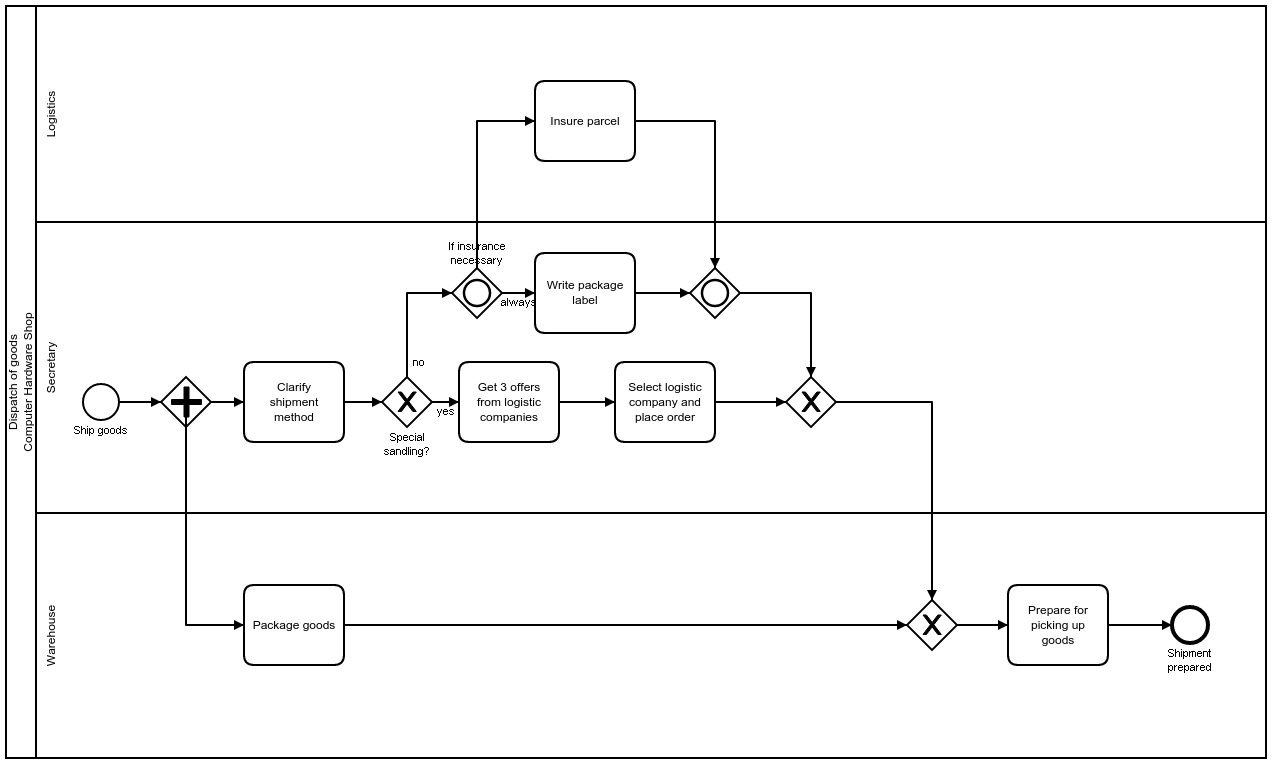
\includegraphics[width=1.3\textwidth]{figures/benchmark/Dispatch-of-goods.png}
\end{figure}

\end{landscape}




\begin{landscape}
\thispagestyle{empty}
\newgeometry{left=1cm, top=9cm}
\section*{Recourse \texttt{[RECO]}}
\begin{figure}[!h]
    \centering
    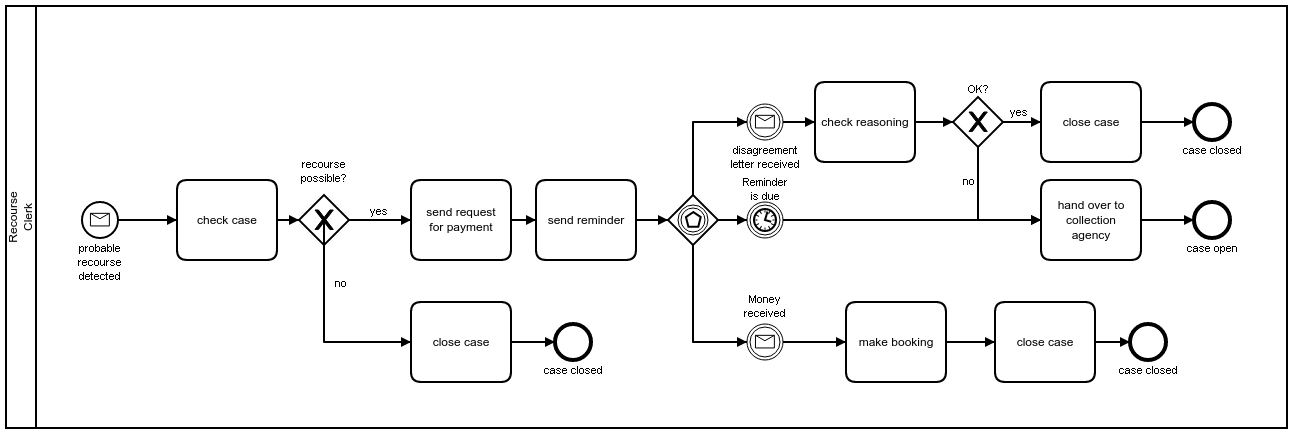
\includegraphics[width=1.3\textwidth]{figures/benchmark/Recourse.png}
\end{figure}
\end{landscape}

\clearpage
%-------------------------


\begin{landscape}
\thispagestyle{empty}
\newgeometry{left=1cm, top=9cm}
\section*{Bicycle Manufacturer \texttt{[BICL]}}
\begin{figure}[!h]
    \centering
    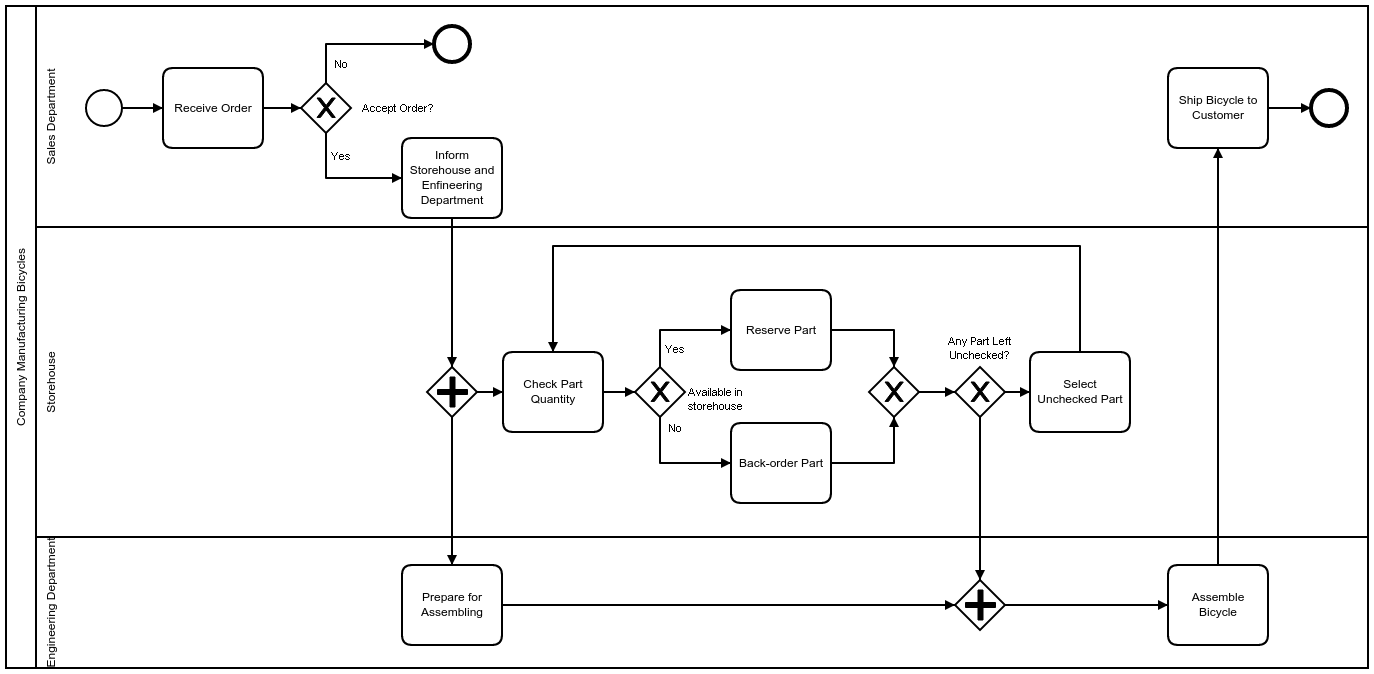
\includegraphics[width=1.3\textwidth]{figures/benchmark/Bicycle_Manufacturer.png}
\end{figure}
\end{landscape}

\clearpage
%-------------------------


\begin{landscape}
\thispagestyle{empty}
\newgeometry{left=1cm, top=9cm}
\section*{Computer Repair Shop \texttt{[COMP]}}
\begin{figure}[!h]
    \centering
    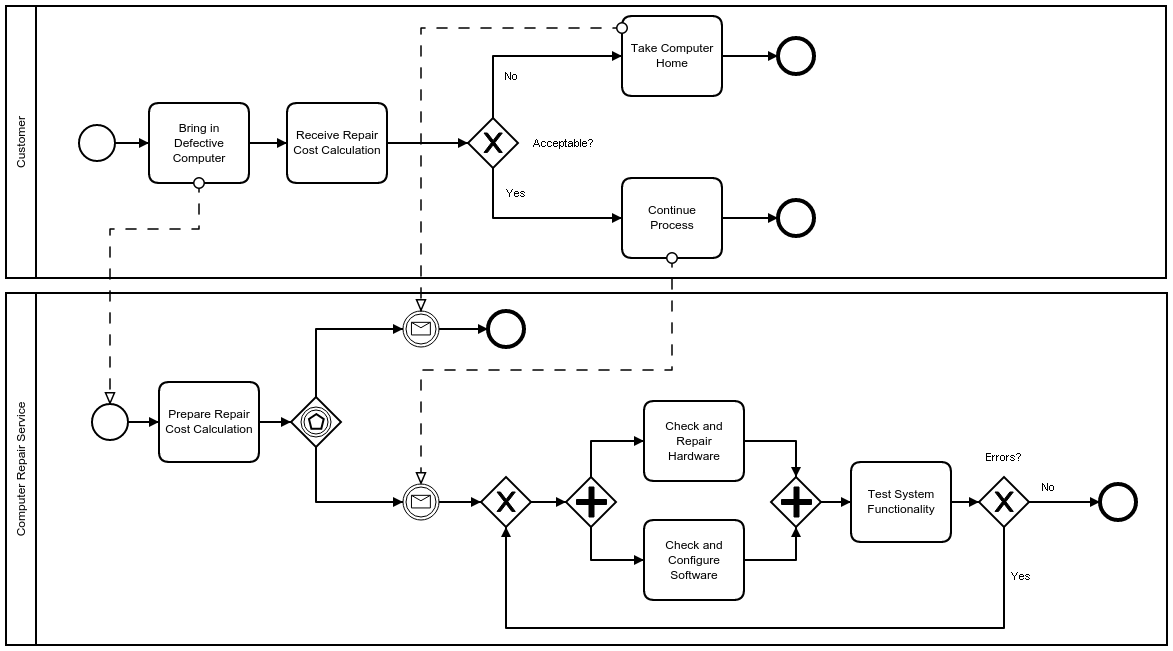
\includegraphics[width=1.3\textwidth]{figures/benchmark/Computer_Repair.png}
\end{figure}
\end{landscape}

\clearpage
%-------------------------


\begin{landscape}
\thispagestyle{empty}
\newgeometry{left=1cm, top=9cm}
\section*{Hotel \texttt{[HOTL]}}
\begin{figure}[!h]
    \centering
    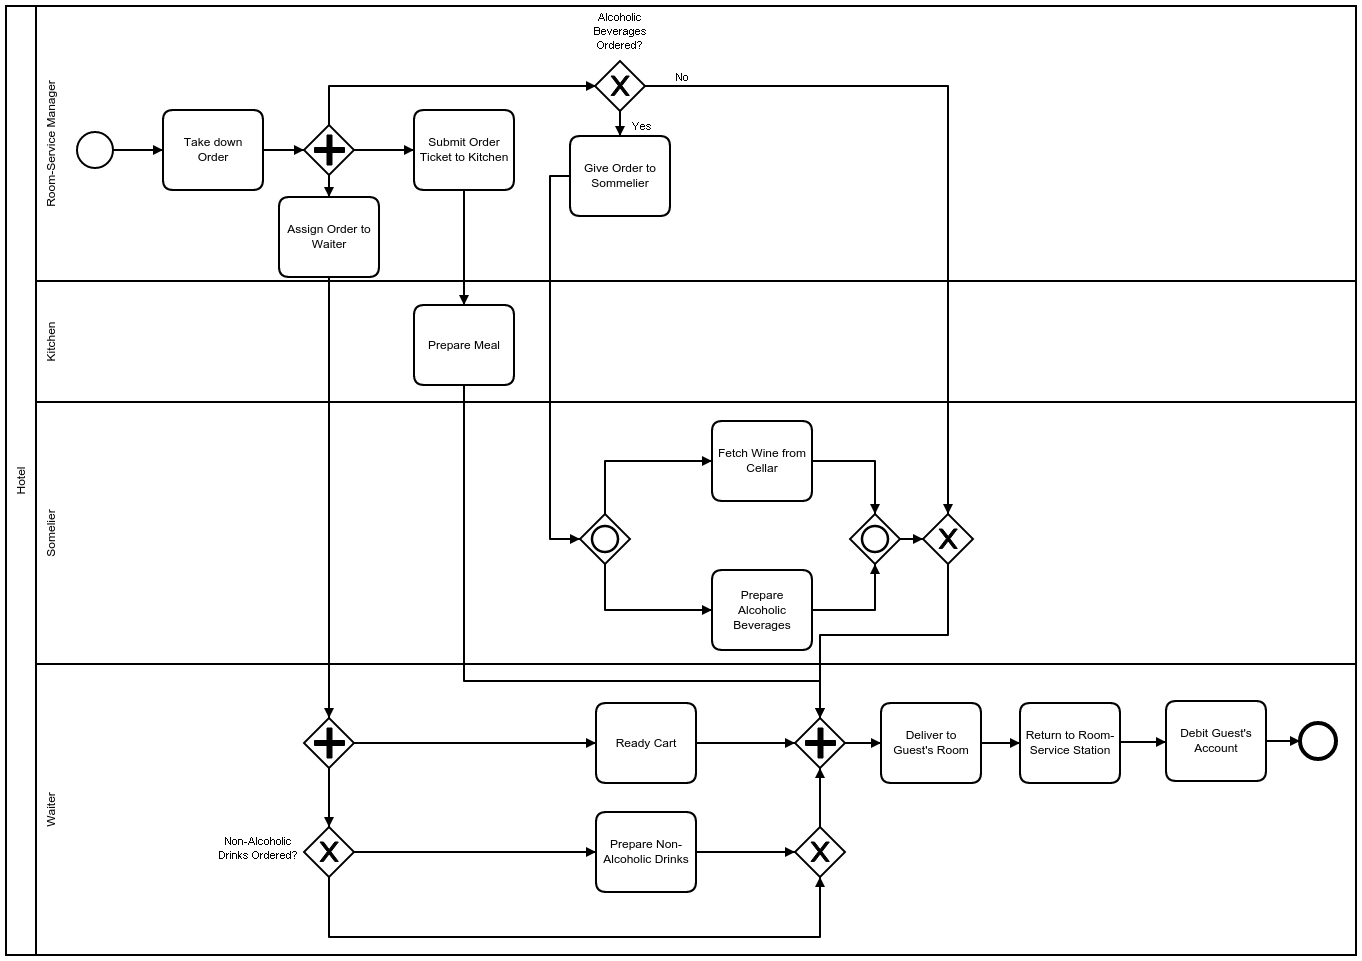
\includegraphics[width=1.3\textwidth]{figures/benchmark/Hotel.png}
\end{figure}
\end{landscape}

\clearpage
%-------------------------


\begin{landscape}
\thispagestyle{empty}
\newgeometry{left=1cm, top=9cm}
\section*{Underwriter \texttt{[UNWR]}}
\begin{figure}[!h]
    \centering
    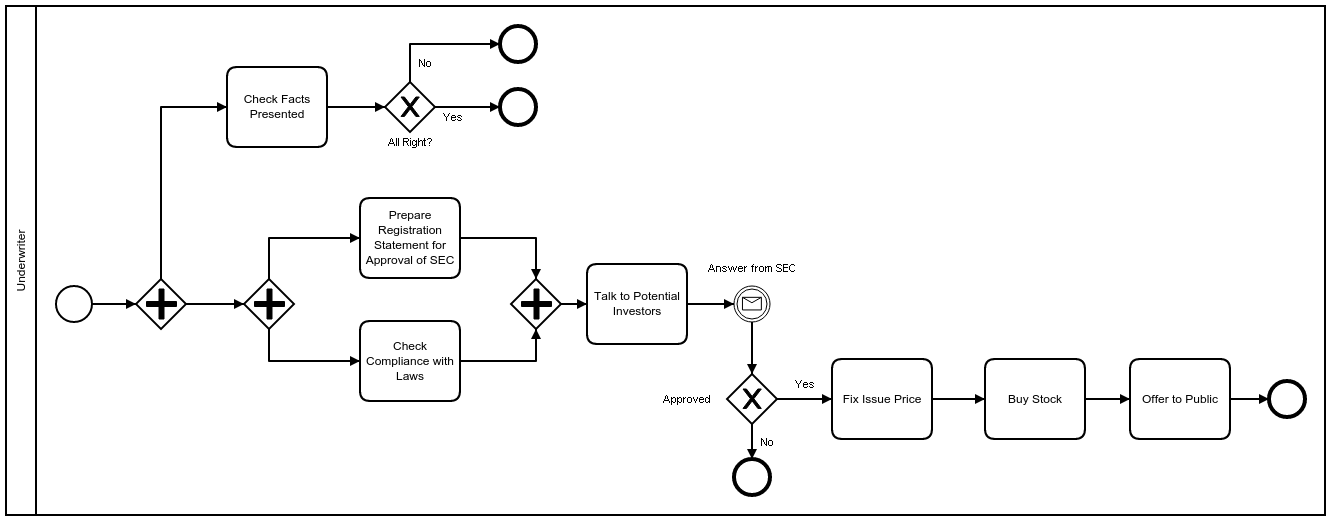
\includegraphics[width=1.3\textwidth]{figures/benchmark/Underwriter.png}
\end{figure}
\end{landscape}

\clearpage
%-------------------------


\begin{landscape}
\thispagestyle{empty}
\newgeometry{left=1cm, top=9cm}
\section*{Hospital \texttt{[HOSP]}}
\begin{figure}[!h]
    \centering
    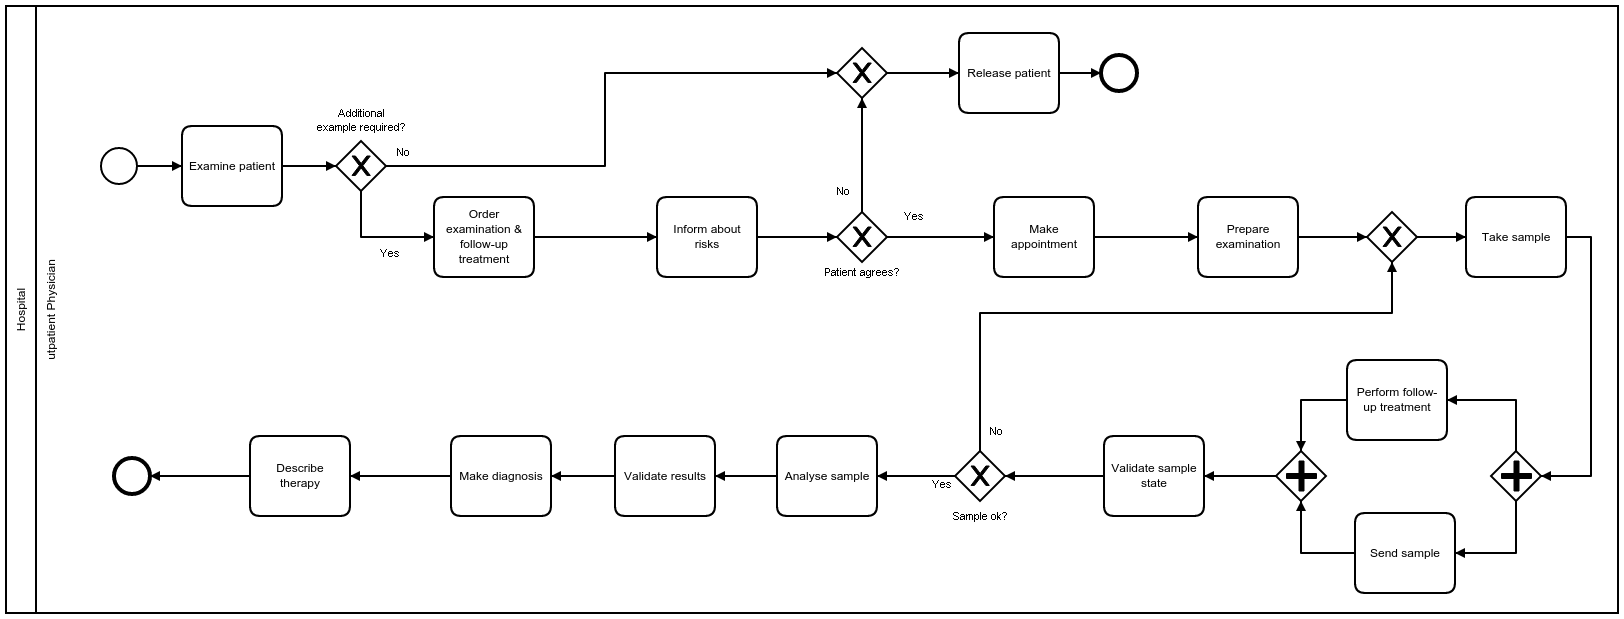
\includegraphics[width=1.3\textwidth]{figures/benchmark/Hospital.png}
\end{figure}
\end{landscape}


\begin{landscape}
\thispagestyle{empty}
\newgeometry{left=1cm, top=9cm}
\section*{Zoo \texttt{[ZOO]}}
\begin{figure}[!h]
    \centering
    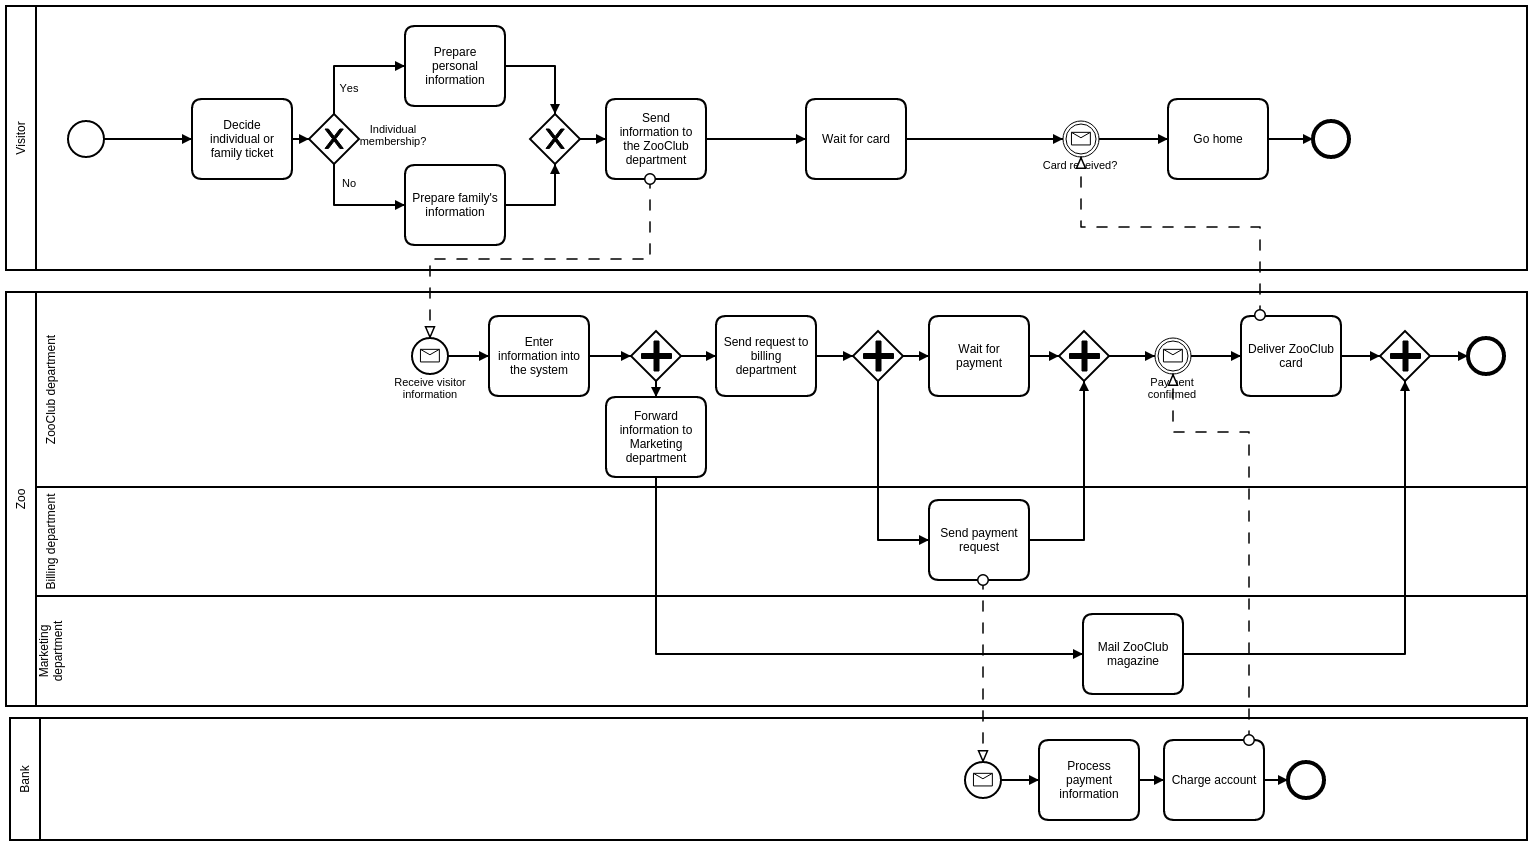
\includegraphics[width=1.3\textwidth]{figures/benchmark/Zoo.png}
\end{figure}
\end{landscape}




